\documentclass{report}
\usepackage[utf8]{inputenc}
\RequirePackage[numbers]{natbib}
\usepackage[intoc,french]{nomencl}
\makenomenclature
\renewcommand{\nomname}{Notations}
\usepackage{etoolbox}
\usepackage{subcaption}
\usepackage{graphicx}

\title{Spécification d'histogrammes dans le cas de zones constantes}
\author{Pierre Dubreuil, Thomas Eboli}

\begin{document}
\maketitle

\begin{abstract}
Dans ce rapport, nous allons présenter nos résultats au sujet d'application de la spécification d'histogrammes au traitement des images. Nous nous sommes appuyé sur le code fourni par madame Nikolova ainsi que sur le papier de base. La première étape du travail, en amont de tout bout de code a été de comprendre les enjeux soulevés par le papier et d'appréhender la puissance du speed-up de la phase "d'ordering" dans le problème de la spécification d'histogrammes. L'un des principaux problèmes que nous avons cherché à résoudre est l'a présence de "large pixels" dans les images obtenues après spécification. Notre méthode de résolution repose sur des considérations probabilistes d'un histogramme comme la distribution de probabilité d'une variable aléatoire $X$ qui est ici l'image.
\end{abstract}

\paragraph*{}
Ce document est organisé comme suit: la partie 1 est dédiée à présenter le problème de "large pixels" et d'en comprendre la source. La partie 2 présente notre approche pour résoudre le problème ainsi que que les résultats obtenus.

\section*{Présentation du problème de "large pixels"}

\begin{figure}
\centering
\begin{minipage}[width=0.5\textwidth]
\centering
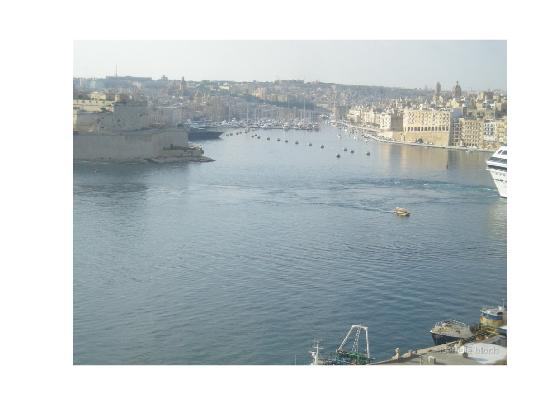
\includegraphics[width=0.75\textwidth]{images/im_x.jpg}
\end{minipage}%
\begin{minipage}[width=0.5\textwidth]
\centering
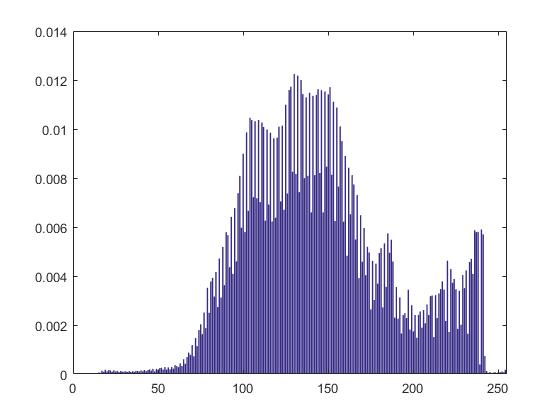
\includegraphics[width=0.75\textwidth]{images/hist_x.jpg}
\end{minipage}
\caption{Image de départ et son histogramme}
\label{fig:im_x}
\end{figure}

\begin{figure}
\centering
\begin{minipage}{width=0.5\textwidth}
\centering
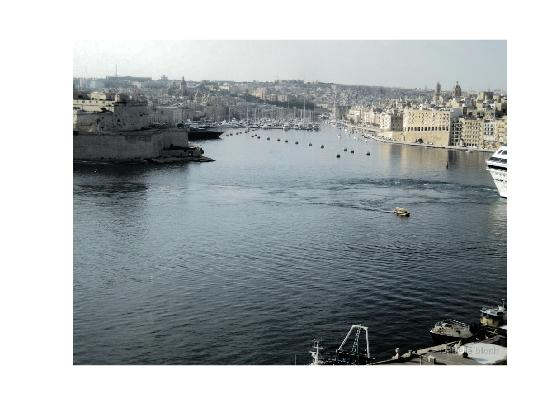
\includegraphics[width=0.75\textwidth]{images/im_xx.jpg}
\end{minipage}%
\begin{minipage}{width=0.5\textwidth}
\centering
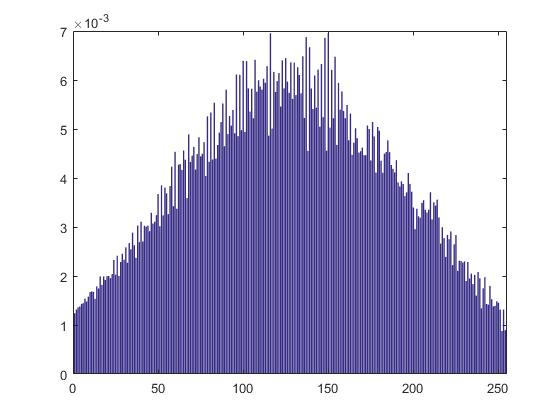
\includegraphics[width=0.75\textwidth]{images/hist_xx.jpg}
\end{minipage}
\caption{Image améliorée obtenue grâce au tri par la procédure order}
\label{fig:im_xx}
\end{figure}

\section*{Résolution par ajout de bruit}
\subsection*{Approche probabiliste}
\paragraph*{}
La partie précédente met en évidence que le transport d'un histogramme d'une image réelle vers un histogramme cible ne peut se faire complètement ce qui laisse apparaître des défauts dans l'image générée à partir du nouvel histogramme obtenu.
\subparagraph*{}
Comme annoncé dans l'introduction, nous sommes partis du constat qu'une image est la réalisation d'une variable aléatoire $X$ vivant dans un espace de très grande dimension (de l'ordre du million en pratique) et que son ou ses histogrammes, selon que X est une image couleur ou en niveau de gris, représentent les distributions de probabilités de chacun des canaux. Dans ce contexte, on peut utiliser un résultat classique de probabilités:
\newline
\paragraph{Théorème 1:} Soient $x$ et $y$ les réalisations de deux variables aléatoires $X$ et $Y$ de densités respectives $f_x$ et $f_y$. Alors $x+y$ est aussi une variable aléatoire suivant la loi $X+Y$ et de densité $f_x * f_y$.
\subparagraph{} Toutes les considérations suivantes seront prises sur des images en niveaux de gris. Pour appliquer les résultats à des images couleurs, il suffit d'appliquer les calculs à chacun des canaux. On considérant maintenant que $x$ est notre image et en notant $b$ le bruit (gaussien, uniforme, peu importe), on obtient que l'image $x_b = x+b$ possède un histogramme qui s'écrit $h_x * h_b$. On peut donc maintenant jouer sur le type de bruit et son écart-type $\sigma$ pour modifier l'allure de l'histogramme  de $x$ et donc modifier en aval le contraste de manière plus fine.
\subparagraph*{} Théoriquement, on arrive alors a moyenner l'histogramme de x. On définit la valeur d'un bin $h_{x_b}(i)$ pour $i \in {0,...,255}$ comme une fonction de de $h_x(i)$ mais aussi de ses voisins. On force donc l'histogramme avoir des valeurs plus faibles aux endroits où il n'y avait pas de pixels au départ ce qui réduit l'apparition de motifs invisible au début et qui deviennent visibles par la suite. Le choix du type de bruit à appliquer définit donc le type de moyenne qu'on utilise. Par exemple un bruit uniforme appliquera une moyenne classique aux bins de l'histogramme de $x$.
\end{document}